\marginnote{\adforn{42} \Chapref{chap:dataset} \hfill \Chapref{chap:mth1} \adforn{43}}

\paragraph{Synopsis}
This chapter introduces … We introduce the types of … in §\ref{sec:res1:sec1}, and we detail each of them in §\ref{sec:sota1:perm}-\ref{sec:sota1:pc}.

% =======================================================

\section{Introduction}
\label{sec:sota1:introduction}

… Another line of comparison emerged through state of the art, concerning the objective of the neural networks, which can either be:
\begin{description}
    \setlength\itemsep{0em}
    \item [Permutation:] Given all the fragments, the neural network predicts a permutation that gives a correct reassembly (§\ref{sec:sota1:perm});
    \item [Pairwise comparison:] The neural network predicts the position of a fragment in relation to another fragment (§\ref{sec:sota1:pc}).
\end{description}

% =======================================================

\section{Permutations}
\label{sec:sota1:perm}

… section intro …

\begin{description}
    \item Noroozi and Favaro\footnote{\citep{noroozi2016unsupervised} M. Noroozi and P. Favaro, \href{https://arxiv.org/pdf/1603.09246.pdf}{Unsupervised learning of visual representations by solving jigsaw puzzles}.} solve \blindtext

    \item Santa Cruz et al.\footnote{\citep{santa2017deeppermnet} R. Santa Cruz et al., \href{https://arxiv.org/pdf/1704.02729.pdf}{DeepPermNet: Visual Permutation Learning}.} propose an architecture that \blindtext

\begin{marginfigure}
    \centering
    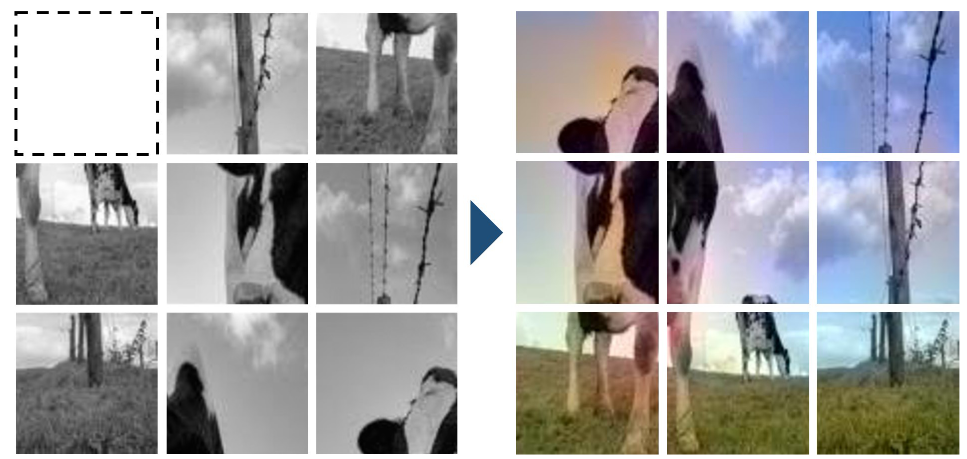
\includegraphics[width=\linewidth]{30-part1/img/kim.jpg}
    \caption[A complex permutation task]{Example of permutation task with inpainting and colorization. ©~Kim et al. \citep{kim2018learning}.}
    \label{fig:soadz:kim}
\end{marginfigure}

    \item Kim et al.\footnote[][1em]{\citep{kim2018learning} D. Kim et al., \href{https://arxiv.org/pdf/1802.01880.pdf}{Learning Image Representations by Completing Damaged Jigsaw Puzzles}.} tackle the case of \blindtext

    \item Wei et al.\footnote{\citep{wei2019iterative} C. Wei et al., \href{https://arxiv.org/pdf/1812.00329.pdf}{Iterative Reorganization with Weak Spatial Constraints: Solving Arbitrary Jigsaw Puzzles for Unsupervised Representation Learning}.} \blindtext
\end{description}

% =======================================================

\section{Pairwise comparison}
\label{sec:sota1:pc}

… section intro …